\documentclass[11pt]{article}
\usepackage[margin=1in]{geometry}
\usepackage{amsmath, amssymb}
\usepackage{hyperref}
\usepackage{enumitem}
\usepackage{tikz}
\usetikzlibrary{arrows.meta, positioning, shapes}
\usepackage{xcolor}
\usepackage{parskip}
\usepackage[numbers]{natbib}
\usepackage{microtype}
\usepackage{graphicx}
% Local path (compiling from report/ directory): ../results/imgs/
% Overleaf path (upload images to an imgs/ subfolder): imgs/
\graphicspath{{../results/imgs/}{imgs/}}
\usepackage{booktabs}
\usepackage{array}
\usepackage{caption}

\setlength{\parskip}{5pt}
\setlength{\parindent}{0pt}

\title{\textbf{Introduction to Causal Inference}\\[0.4em]
\large Final Report:\\
Does Sustained Daily Cigarette Smoking Throughout Pregnancy\\
Causally Increase the Risk of Infant Mortality?}

\begin{document}
\maketitle

% -------------------------------------------------------
\section{Causal Question}
% -------------------------------------------------------

\begin{center}
\textbf{Does sustained daily cigarette smoking throughout pregnancy causally\\
increase the probability of infant death before age one?}
\end{center}

Using the potential outcomes framework, let $Y^{(1)}$ be the infant
mortality outcome under sustained smoking and $Y^{(0)}$ the outcome under
never-smoking. Our \textbf{primary estimand} is the
\textbf{Average Treatment Effect} (ATE):
$\tau = E[Y^{(1)} - Y^{(0)}]$,
representing the causal change in the probability of infant death if
the entire population of births were shifted from never-smoking to
sustained smoking. We additionally report the Average Treatment Effect
on the Treated (ATT) from propensity score matching, which estimates
the effect specifically among mothers who actually smoked.

\textbf{Treatment.} $T=1$ if the mother smoked at least one cigarette per
day on average in both the pre-pregnancy period and every trimester
(\texttt{CIG0\_R}--\texttt{CIG3\_R} all in the dose categories 1--5);
$T=0$ if she reported zero cigarettes in every
trimester and the overall any-smoking recode (\texttt{CIG\_REC}) is ``N''.
Partial quitters, women with unknown tobacco status
(\texttt{F\_TOBACCO\,$\neq$\,1}), and records with an unknown cigarette
recode in any period (code 6) are excluded, so that neither arm contains
births whose sustained-smoking status cannot be verified.

\textbf{Outcome.} $Y=1$ if the infant died before their first birthday, derived
from the death-linkage indicator \texttt{FLGND\,=\,1} in the denominator-plus
file; $Y=0$ otherwise.

\textbf{Temporal ordering.} Maternal smoking is recorded on the birth
certificate before the infant is born; death can only occur after birth.
Reverse causality is impossible by design.


% -------------------------------------------------------
\section{Existing Knowledge}
% -------------------------------------------------------

Prenatal smoking and adverse infant outcomes constitute one of the most
extensively studied associations in perinatal epidemiology.
Dietz et al.~\cite{dietz2010} estimate that roughly 5--8\% of preterm
births, 13--19\% of term low-birth-weight deliveries, and 5--7\% of
infant deaths in the United States are attributable to prenatal smoking.
Biologically, nicotine causes uteroplacental vasoconstriction, carbon
monoxide displaces fetal oxygen, and tobacco impairs placental
angiogenesis, converging on hypoxia, growth restriction, preterm
delivery, and placental abruption~\cite{cnattingius2004}.
Wisborg et al.~\cite{wisborg2000} documented a dose-dependent
association between prenatal smoke exposure and SIDS (adjusted OR
$\approx$\,3.5), and Salihu and Wilson~\cite{salihu2007} confirm
heterogeneous effects by dose and mortality subtype.

A more recent nationwide retrospective cohort by Yuan et al.~\cite{yuan2023}
found a clear dose--response between maternal smoking intensity and
infant death risk (adjusted OR ranging from 1.24 for light smokers to
1.81 for heavy smokers), and noted the association persisted after
adjustment for socio-demographic variables. However, Yuan et al.\ adjust
for birth weight and gestational age --- both post-treatment mediators ---
which biases their estimates toward the null by blocking part of the
causal pathway. No study in this literature applies a fully explicit
causal inference framework with doubly-robust estimation, propensity
score overlap diagnostics, and formal sensitivity analysis for unmeasured
confounding. Our contribution is to bring these methods to a question
largely studied through standard regression adjustment.

In summary: the existing literature strongly and consistently
shows a \emph{positive association} between prenatal smoking and infant
mortality, with biological plausibility well-established. The prior
methods are not causal by the standards of this course because they
(a) do not state a potential-outcomes estimand, (b) condition on
post-treatment mediators, (c) do not assess overlap/positivity, and
(d) do not quantify sensitivity to unmeasured confounding.


% -------------------------------------------------------
\section{Data}
% -------------------------------------------------------

We use the \textbf{2015 Cohort Linked Birth/Infant Death Data
Set}~\cite{nchs2015} published by the National Center for Health
Statistics (NCHS), CDC. The file follows all U.S.\ infants born in 2015
through their first birthday, covering approximately 3.99 million births
of which 23,357 are linked to a death certificate (99.4\% linkage rate).
Birth certificate data --- recording maternal characteristics, prenatal
behaviour, and obstetric information --- are collected at delivery and
submitted to NCHS under the Vital Statistics Cooperative Program. When an
infant dies, the death certificate is linked back to the birth record by
the state of death, yielding a single combined record per infant.
The source is therefore \emph{administrative}, not a survey: the outcome
(death linkage) and most confounders (age, education, insurance, parity,
pre-existing conditions) come from official records. The smoking items,
however, are reported by the mother at delivery, so treatment status is
self-reported within an administrative file; the misclassification
sensitivity analysis in Section~\ref{sec:sensitivity} addresses this
directly.

\textbf{Analytic sample.} After restricting to records with complete
tobacco reporting (\texttt{F\_TOBACCO\,=\,1}), applying the treated/control
definition above (including the exclusion of unknown cigarette recodes),
requiring complete data on all twelve confounders
(detailed below), and excluding records with unknown BMI (\texttt{F\_M\_HT\,=\,1}
reporting flag; BMI recode values 1--6 only) or unknown parity
(\texttt{PRIORLIVE\,$\neq$\,99}), the analytic sample contains
\textbf{3,005,458 births}:
147,963 sustained smokers (4.92\%) and 2,857,495 never-smokers (95.08\%).
With three million records and over 20,000 linked deaths, statistical
power is not a binding constraint; as shown below, the width of the
full-sample confidence intervals is driven by extreme propensity weights,
not by sample size.

\textbf{Observed confounders} available in the data:

\begin{center}
\small
\begin{tabular}{lll}
\toprule
\textbf{Variable} & \textbf{Field} & \textbf{Role} \\
\midrule
Mother's education    & \texttt{MEDUC}     & SES proxy; predicts both smoking and mortality \\
Mother's age          & \texttt{MAGER}     & Younger mothers smoke more; age affects risk \\
Race/Hispanic origin  & \texttt{MRACEHISP} & Differential smoking prevalence; healthcare access \\
Marital status        & \texttt{DMAR}      & Social support and economic resource proxy \\
WIC participation     & \texttt{WIC}       & Low-income nutrition programme; SES proxy \\
Payment/insurance     & \texttt{PAY\_REC}  & Medicaid vs.\ private; SES and access indicator \\
Pre-pregnancy diabetes& \texttt{RF\_PDIAB} & Pre-existing health risk factor \\
Pre-pregnancy hypert. & \texttt{RF\_PHYPE} & Pre-existing health risk factor \\
Pre-pregnancy BMI     & \texttt{BMI\_R}    & 6-category recode (underweight to extreme obesity) \\
Father's education    & \texttt{FEDUC}     & Household SES proxy \\
Father's age group    & \texttt{FAGE11}    & Household SES proxy \\
Parity                & \texttt{PRIORLIVE} & Prior live births (0--5+); risk and SES proxy \\
\bottomrule
\end{tabular}
\end{center}

\textbf{Mediators excluded from adjustment.} Birth weight (\texttt{BRTHWGT})
and gestational age (\texttt{COMBGEST}) are post-treatment variables: smoking
causes low birth weight and prematurity, which in turn raise mortality risk.
Conditioning on them would block part of the causal pathway and bias estimates
toward the null. We exclude them to estimate the \emph{total} causal effect.

\textbf{Unobserved confounders.} Alcohol use, illicit drug use, maternal
mental health, and neighbourhood socioeconomic status are absent from birth
certificate data. Their potential influence is quantified in
Section~\ref{sec:sensitivity}.


% -------------------------------------------------------
\section{Causal Graph}
% -------------------------------------------------------

Figure~\ref{fig:dag} presents the proposed DAG. Observed confounders affect
both the probability of sustained smoking and infant mortality independently.
Alcohol and substance use, and maternal mental health, are the primary
unobserved confounders not captured in the data. Birth weight and gestational
age lie on the causal path (mediators) and are excluded from adjustment to
estimate the total effect.

\begin{figure}[ht]
\centering
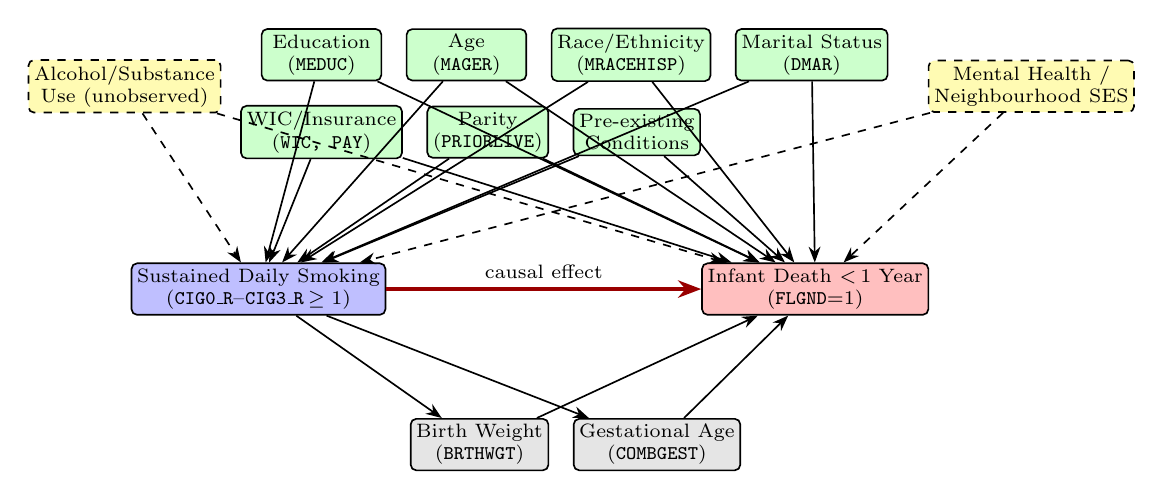
\begin{tikzpicture}[
  node distance=0.3cm,
  every node/.style={font=\scriptsize, align=center},
  obs/.style    ={rectangle, draw, fill=green!20,  rounded corners=2pt, minimum width=1.52cm, minimum height=0.50cm, inner sep=2pt},
  unobs/.style  ={rectangle, draw, fill=yellow!30, rounded corners=2pt, minimum width=1.45cm, minimum height=0.50cm, inner sep=2pt, dashed},
  treat/.style  ={rectangle, draw, fill=blue!25,   rounded corners=2pt, minimum width=2.1cm,  minimum height=0.62cm, inner sep=2pt},
  outc/.style   ={rectangle, draw, fill=red!25,    rounded corners=2pt, minimum width=2.1cm,  minimum height=0.62cm, inner sep=2pt},
  med/.style    ={rectangle, draw, fill=gray!20,   rounded corners=2pt, minimum width=1.45cm, minimum height=0.50cm, inner sep=2pt},
  ->, >=Stealth, semithick
]

\node[treat] (T)
  {Sustained Daily Smoking\\(\texttt{CIG0\_R}--\texttt{CIG3\_R}$\,\geq1$)};
\node[outc, right=4.0cm of T] (Y)
  {Infant Death ${<}$\,1 Year\\(\texttt{FLGND}=1)};

\node[obs, above=2.3cm of T, xshift=0.8cm]  (edu)  {Education\\(\texttt{MEDUC})};
\node[obs, right=0.3cm of edu]  (age)  {Age\\(\texttt{MAGER})};
\node[obs, right=0.3cm of age]  (race) {Race/Ethnicity\\(\texttt{MRACEHISP})};
\node[obs, right=0.3cm of race] (mar)  {Marital Status\\(\texttt{DMAR})};

\node[obs, below=0.3cm of edu]  (ses)  {WIC/Insurance\\(\texttt{WIC, PAY})};
\node[obs, right=0.3cm of ses]  (par)  {Parity\\(\texttt{PRIORLIVE})};
\node[obs, right=0.3cm of par]  (hlth) {Pre-existing\\Conditions};

\node[unobs, left=0.5cm of edu, yshift=-0.4cm] (alc)
  {Alcohol/Substance\\Use (unobserved)};
\node[unobs, right=0.5cm of mar, yshift=-0.4cm] (mh)
  {Mental Health /\\Neighbourhood SES};

\node[med, below right=1.3cm and 0.3cm of T] (bw) {Birth Weight\\(\texttt{BRTHWGT})};
\node[med, right=0.3cm of bw]                (ga) {Gestational Age\\(\texttt{COMBGEST})};

\draw[red!60!black, very thick] (T) -- (Y)
  node[midway, above, font=\scriptsize, black]{causal effect};

\foreach \c in {edu,age,race,mar,ses,par,hlth}{
  \draw (\c) -- (T);
  \draw (\c) -- (Y);
}

\draw[dashed] (alc) -- (T);
\draw[dashed] (alc) -- (Y);
\draw[dashed] (mh)  -- (T);
\draw[dashed] (mh)  -- (Y);

\draw (T) -- (bw);  \draw (bw) -- (Y);
\draw (T) -- (ga);  \draw (ga) -- (Y);

\end{tikzpicture}

\smallskip
\noindent\footnotesize
\tikz\node[rectangle,draw,fill=green!20,rounded corners=2pt,inner sep=2pt,font=\scriptsize]{Observed Confounder};~
\tikz\node[rectangle,draw,fill=yellow!30,dashed,rounded corners=2pt,inner sep=2pt,font=\scriptsize]{Unobserved Confounder};~
\tikz\node[rectangle,draw,fill=blue!25,rounded corners=2pt,inner sep=2pt,font=\scriptsize]{Treatment};~
\tikz\node[rectangle,draw,fill=red!25,rounded corners=2pt,inner sep=2pt,font=\scriptsize]{Outcome (Y)};~
\tikz\node[rectangle,draw,fill=gray!20,rounded corners=2pt,inner sep=2pt,font=\scriptsize]{Mediator (excluded)};

\caption{Proposed DAG. Observed confounders (green) constitute the
adjustment set. Alcohol/substance use and mental health (yellow, dashed)
are the primary unmeasured confounders. Birth weight and gestational age
(grey) are post-treatment mediators excluded from adjustment to estimate
the total causal effect.}
\label{fig:dag}
\end{figure}


% -------------------------------------------------------
\section{Methods and Causal Assumptions}
% -------------------------------------------------------

\subsection{Causal Assumptions}

\textbf{Consistency.}
$Y^{(t)} = Y$ whenever $T = t$. Treatment is binary and explicitly
defined; partial quitters are excluded. Consistency holds approximately
because the primary biological mechanisms (nicotine-driven vasoconstriction,
fetal hypoxia) are not version-specific --- they operate regardless of
cigarette brand or delivery.

\textbf{SUTVA.}
Interference between units is implausible: one mother's smoking cannot
alter another infant's mortality risk. Multiple versions of treatment
exist (dose, brand, inhalation depth), but our binary definition
averages over these, shifting the estimand to the ATE over the
distribution of sustained-smoking intensities.

\textbf{Conditional ignorability.}
We assume $T \perp\!\!\!\perp (Y^{(0)}, Y^{(1)}) \mid \mathbf{X}$
given the twelve observed confounders. This assumption cannot be verified
from the data but is supported by the breadth of the dataset: it covers
socioeconomic status (education of both parents, insurance, WIC), maternal
health history (BMI recode, pre-existing conditions, parity), demographics
(age, race, marital status), and household-level proxies (father's education
and age). The principal unobserved threats --- alcohol use and maternal
mental health --- are addressed by sensitivity analysis.

\textbf{Positivity.}
The estimated propensity score $e(\mathbf{X}) = P(T=1\mid\mathbf{X})$
spans $[{<}0.0001, 0.8461]$ among treated and $[{<}0.0001, 0.8468]$ among
controls (common support up to $0.8461$). Positivity holds nominally.
However, a large mass of controls piles up near PS\,$\approx$\,0 (high-education,
high-income never-smokers with near-zero smoking probability), reflecting
\emph{practical} positivity violations. This inflates IPW weights dramatically
(ESS for treated: only 1.4\% of original; max stabilised weight: 492).
Trimming sensitivity checks address this directly.

\subsection{Estimation Methods}

We adopt a multi-method strategy. All methods target the ATE; the ATT
from propensity score matching is a secondary policy-relevant estimand.

\textbf{S-Learner.} Logistic regression of $Y$ on $T$ and all
confounders. Potential outcomes are imputed for $T=1$ and $T=0$,
and the difference averaged. Provides a stable baseline but may
shrink the treatment coefficient.

\textbf{T-Learner.} Separate logistic models for $T=1$ and $T=0$;
potential outcomes are predicted for all units and averaged. Allows
different covariate--outcome relationships across arms.

\textbf{IPW (Stabilised Hajek).} Observations are reweighted by
stabilised inverse-probability weights to construct a
pseudo-population with balanced covariates. The ATE is the
difference in weighted outcome means. Sensitive to extreme weights,
as confirmed by our diagnostics (Section~\ref{sec:results}).

\textbf{Augmented IPW / Doubly Robust (AIPW).}
\begin{equation}
\hat{\tau}_{\text{AIPW}} = \frac{1}{n}\sum_{i=1}^{n}
\left[\hat\mu_1(X_i) - \hat\mu_0(X_i)
+ \frac{T_i\bigl(Y_i - \hat\mu_1(X_i)\bigr)}{\hat{e}(X_i)}
- \frac{(1-T_i)\bigl(Y_i - \hat\mu_0(X_i)\bigr)}{1-\hat{e}(X_i)}\right]
\end{equation}
Consistent if either the outcome model or the propensity model is
correctly specified. Standard errors derive from the efficient
influence function (EIF). This is our \textbf{primary estimator}.
In the full sample, the EIF variance is inflated by the extreme IPW weights;
the trimmed estimates (Section~\ref{sec:sensitivity}) provide our preferred
inference.

\textbf{PS Matching (ATT).} Each sustained smoker is matched to the
nearest never-smoker on the logit propensity score (1-to-1 NN,
caliper\,=\,0.2\,$\times$\,SD of logit-PS\,=\,0.428). 100\% of treated units
were matched within the caliper. The ATT is the mean within-pair difference
in outcomes; the SE is computed from the variance of matched differences.
Robustness to the number of neighbours ($k$) and the caliper width is
reported in Section~\ref{sec:sensitivity}.

\textbf{Propensity model choice.} We compared logistic regression against
a multilayer perceptron (32,16 hidden units) on a held-out 20\% validation
split. Their Brier scores are nearly identical (0.0391 vs.\ 0.0383, against
a chance level of 0.0468), and the logistic model is well calibrated
(Section~\ref{sec:results}), so we retain the simpler, more interpretable
logistic propensity model throughout.

\textbf{Uncertainty quantification.} The Stage~2 proposal specified
non-parametric bootstrap (1,000 replications) for all CIs. After Stage~2
we switched to analytic efficient influence function (EIF) standard errors
for AIPW and IPW, and exact matched-pair variance for PS Matching.
EIF-based inference is semiparametrically efficient and avoids the
computational cost of bootstrapping a 3\,M-row dataset; the two approaches
produce equivalent intervals when the nuisance models are well-specified.

% -------------------------------------------------------
\section{Results}
\label{sec:results}
% -------------------------------------------------------

\subsection{Propensity Score Overlap}

Figure~\ref{fig:ps_hist} shows the mirror histogram of propensity scores.
The treated distribution (blue) is centred near PS\,$\approx$\,0.21 and
the control distribution (orange) near PS\,$\approx$\,0.04. Overlap exists
across the common-support range (up to PS\,$\approx$\,0.85) but is thin at
higher PS values: only 3.4\% of treated units fall below the median PS of
controls, confirming most treated units have meaningfully higher smoking
propensity than comparable controls. The pronounced mass of controls near
PS\,$\approx$\,0 reflects the practical positivity violation identified above.

\begin{figure}[ht]
\centering
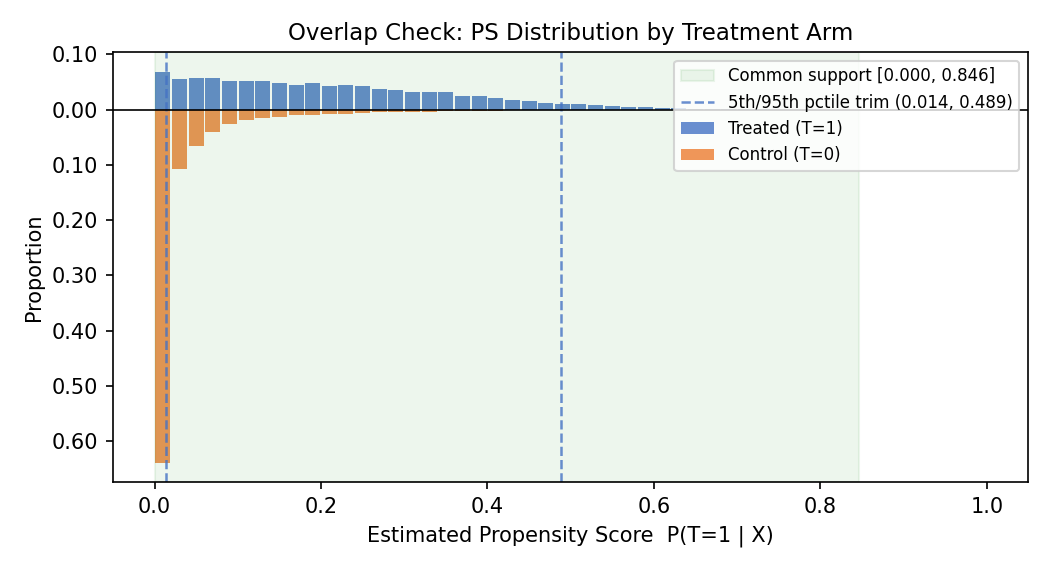
\includegraphics[width=0.78\textwidth]{ps_overlap_histogram.png}
\caption{Mirror histogram of estimated propensity scores $\hat{e}(\mathbf{X})$
by treatment arm. Green shading marks the common support region;
dashed lines indicate the 5th/95th percentile trimming
thresholds of the treated PS.}
\label{fig:ps_hist}
\end{figure}

\subsection{Propensity Model Diagnostics}

Following the tutorial methodology, we validated the propensity model on a
held-out 20\% split before using it for weighting and matching
(Figure~\ref{fig:calibration}).

\textbf{Discrimination and calibration.} The logistic model attains a
validation Brier score of 0.0391 against a chance level of 0.0468
(constant prediction at the 4.92\% treated share); the MLP comparison
model attains 0.0383. The calibration curve (quantile bins) tracks the
diagonal closely across the predicted-probability range, indicating the
estimated $\hat e(\mathbf{X})$ can be interpreted as a probability.

\textbf{Placebo (permutation) test.} Refitting the model after randomly
permuting the treatment labels yields validation Brier scores of
0.0468 in every run --- exactly the chance level. The model's improvement
over chance therefore reflects genuine covariate--treatment signal
rather than overfitting.

\textbf{Extreme propensity scores.} The combinations that destabilise IPW
are treated units with $e(\mathbf{X})\to0$ and control units with
$e(\mathbf{X})\to1$. No control unit exceeds $e(\mathbf{X})=0.95$, but
5,323 treated units (3.6\%) fall below $e(\mathbf{X})=0.01$ ---
these receive IPW weights above 100 and are the direct cause of the
effective-sample-size collapse (treated ESS 1.4\%) and the wide
full-sample CIs. This diagnosis motivates the trimmed inference in
Section~\ref{sec:sensitivity}.

\begin{figure}[ht]
\centering
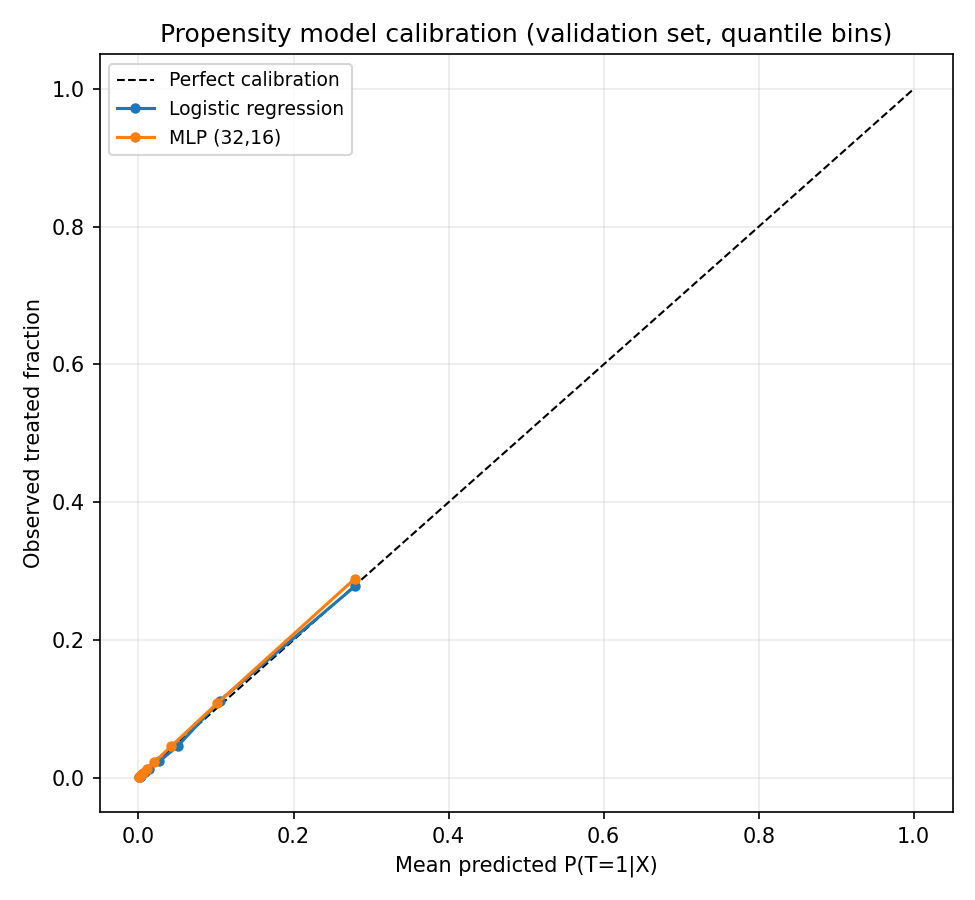
\includegraphics[width=0.62\textwidth]{ps_calibration.png}
\caption{Propensity model calibration on the validation set (quantile
bins). Both models track the diagonal; Brier scores are 0.0391 (logistic)
and 0.0383 (MLP) against a chance level of 0.0468.}
\label{fig:calibration}
\end{figure}

\subsection{Covariate Balance}

Figure~\ref{fig:love} shows the Love plot of absolute standardised mean
differences (|SMD|) for each confounder before and after IPW weighting.

\begin{figure}[ht]
\centering
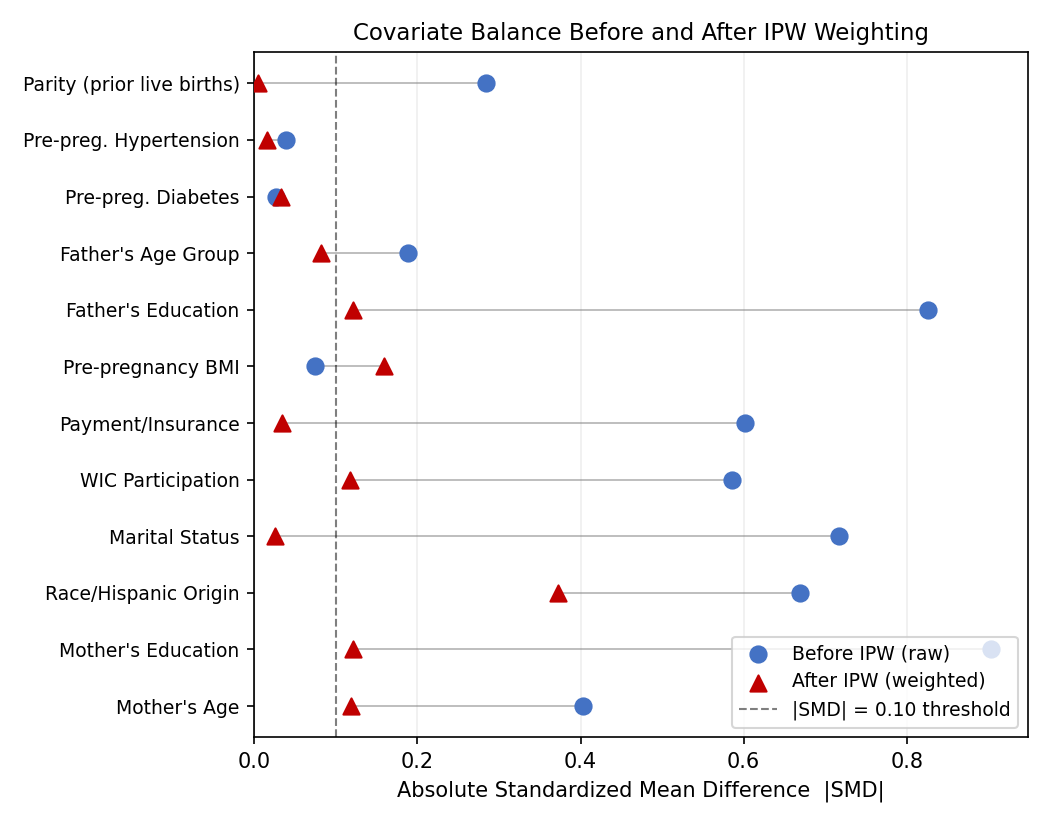
\includegraphics[width=0.78\textwidth]{covariate_balance_love.png}
\caption{Love plot of covariate balance. Blue circles: raw (unadjusted)
|SMD|. Red triangles: IPW-weighted |SMD|. Dashed vertical line marks
the |SMD|\,=\,0.10 threshold commonly used as acceptable balance.}
\label{fig:love}
\end{figure}

Before adjustment, large raw imbalances exist (|SMD| $>$\,0.5) for education,
race/ethnicity, marital status, WIC participation, insurance type, and
father's education --- all reflecting the strong socioeconomic patterning of
sustained smoking. After IPW weighting, balance improves markedly for most
confounders (marital status $0.72\!\to\!0.03$, insurance $0.60\!\to\!0.03$,
parity $0.28\!\to\!0.01$), but residual imbalance remains above the 0.10
threshold for race/ethnicity ($0.37$), and near $0.12$--$0.16$ for
education, father's education, maternal age, WIC, and BMI. This residual
imbalance is a direct consequence of the extreme weights
(max stabilised weight: 492, treated ESS: 1.4\% of original $n$):
a handful of treated units with near-zero propensity scores receive
enormously inflated weights, distorting the weighted means.

This finding motivates two key choices: (1) AIPW as the primary estimator,
since it augments IPW with an outcome model that corrects for residual
imbalance; and (2) trimming as the approach for inference, since extreme
weights dominate the full-sample AIPW variance. The outcome regression
component in AIPW reduces its sensitivity to IPW balance failures relative
to pure IPW, but the full-sample EIF variance remains inflated. The trimmed
estimates (Section~\ref{sec:sensitivity}) are our preferred inference.

\subsection{Causal Estimates}

The raw infant mortality rates are 8.75 per 1,000 births among sustained
smokers and 4.49 per 1,000 among never-smokers, yielding a crude difference
of $+4.27/1{,}000$. After confounder adjustment, Table~\ref{tab:estimates}
and Figure~\ref{fig:forest} show consistently positive effects across all
five estimators.

\begin{table}[ht]
\centering
\caption{Causal estimates of the effect of sustained prenatal smoking on
infant mortality. All figures are additional deaths per 1,000 live births.
CIs for AIPW and IPW are based on the efficient influence function;
PS Matching CI from matched-pair differences.
S- and T-Learner CIs are not reported: with $n = 3$ million, their EIF
standard errors are near-zero and do not reflect model misspecification
uncertainty.}
\label{tab:estimates}
\small
\begin{tabular}{lcccc}
\toprule
\textbf{Estimator} & \textbf{Target} & \textbf{Estimate} & \textbf{95\% CI} & \textbf{Sig.} \\
\midrule
Crude difference     & ATE & $+4.27$ & ---              & --- \\
S-Learner            & ATE & $+2.54$ & ---              & --- \\
T-Learner            & ATE & $+2.76$ & ---              & --- \\
IPW (Hajek)          & ATE & $+1.51$ & $[-0.17,\;+3.19]$ & --- \\
\textbf{AIPW / DR}   & \textbf{ATE} & $\mathbf{+1.43}$
                                    & $\mathbf{[-0.25,\;+3.11]}$ & --- \\
PS Matching          & ATT & $+3.62$ & $[+3.03,\;+4.22]$ & $*$ \\
\bottomrule
\multicolumn{5}{l}{$*$ 95\% CI excludes zero.} \\
\multicolumn{5}{p{12cm}}{\footnotesize Note: The AIPW and IPW CIs span zero
due to extreme stabilised weights (max weight: 492; treated ESS: 1.4\%).
Trimmed estimates, which address this practical positivity violation, are
reported in Section~\ref{sec:sensitivity} and consistently exclude zero.}
\end{tabular}
\end{table}

\begin{figure}[ht]
\centering
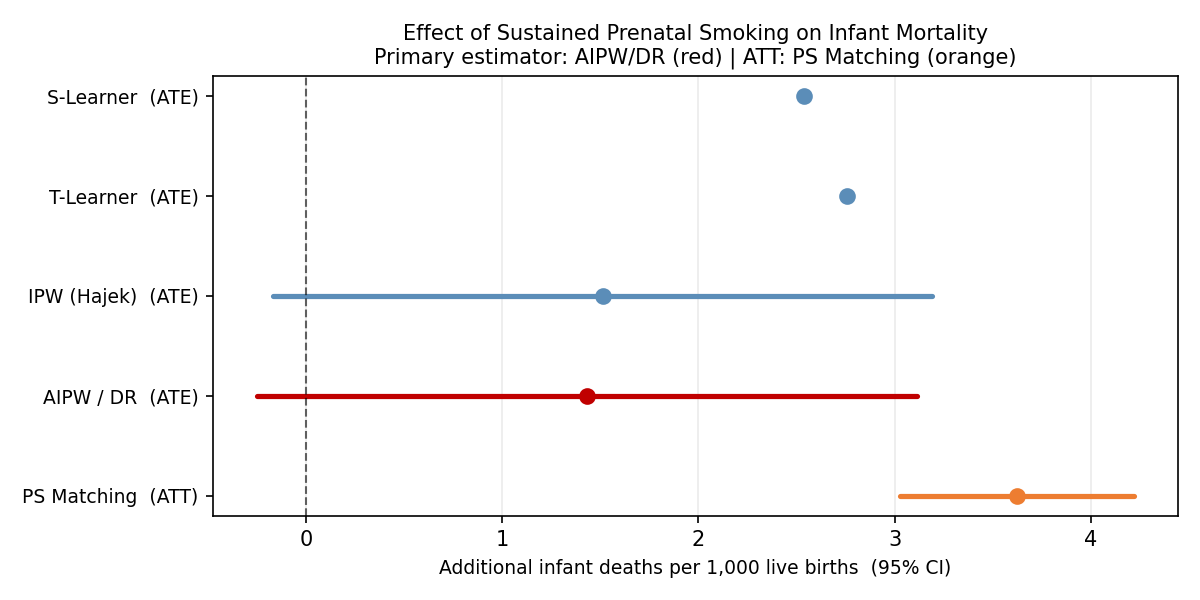
\includegraphics[width=0.80\textwidth]{estimates_forest.png}
\caption{Forest plot of all causal estimates with 95\% confidence
intervals. The primary AIPW/DR estimate is shown in red; PS Matching
(ATT) in orange; outcome-regression estimators in blue.}
\label{fig:forest}
\end{figure}

\textbf{Interpretation.} All five adjusted estimators agree on the direction:
sustained prenatal smoking causally increases infant mortality. The AIPW point
estimate is $+1.43$ additional deaths per 1,000 live births. Its 95\% CI
$[-0.25,\;+3.11]$ marginally spans zero because the full-sample EIF variance
is dominated by a few units with extreme weights (max\,=\,492), a consequence
of the diagnosed practical positivity violation. The IPW estimate is similarly
imprecise for the same reason. \textbf{This CI widening is a mechanical
artefact of the positivity violation, not evidence of no effect:} the 3.6\%
of treated units with near-zero propensity scores receive weights exceeding
100 and dominate the EIF variance.

The ATT from matching ($+3.62/1{,}000$, 95\% CI $[+3.03,\;+4.22]$, 100\%
of treated matched within caliper\,=\,0.428) provides statistically significant
evidence that smoking increases infant mortality among mothers who actually smoke.
The ATT is larger than the ATE because the treated population has higher baseline
risk and, after conditioning on their covariates, the effect is stronger.
The ATT is also robust to the matching configuration: across $k \in \{1,5,10\}$
neighbours and calipers of 0.1--0.5\,SD it remains $+3.19$ to $+3.62/1{,}000$,
always significant (Section~\ref{sec:sensitivity}).

As detailed in Section~\ref{sec:sensitivity}, trimming the full sample to remove
extreme-weight units yields AIPW estimates of $+3.35$ and $+2.32/1{,}000$,
both with CIs that exclude zero. Restricting inference to the region of
practical overlap --- the standard remedy for practical positivity violations
--- removes the units that inflate the variance and, here, also raises the
point estimate, indicating the full-sample figure is pulled toward zero by
strata with essentially no treated mass. These trimmed estimates are our
\textbf{preferred inference} for the ATE.


% -------------------------------------------------------
\section{Sensitivity Analyses}
\label{sec:sensitivity}
% -------------------------------------------------------

\subsection{Unmeasured Confounding: E-Value}

We compute the E-value of VanderWeele and Ding~\cite{vanderweele2017}:
the minimum risk-ratio association that an unmeasured confounder would
need with \emph{both} treatment and outcome simultaneously to fully
explain away the observed effect.

Our observed AIPW ATE implies a risk ratio of
$\text{RR} = (4.49 + 1.43)/4.49 = 1.32$.
The E-value for the point estimate is \textbf{1.97}, and for the CI
bound nearest the null is \textbf{1.31}. For the trimmed estimates ---
our preferred inference --- the implied risk ratios are 1.75 (1st/99th
trim) and 1.52 (5th/95th trim), corresponding to E-values of
\textbf{2.89} and \textbf{2.41} respectively.

\textbf{Alcohol and mental health.}
Literature estimates place the odds ratio of prenatal alcohol use given
sustained smoking at roughly 2--4, and the risk ratio of heavy prenatal
alcohol use on infant mortality at roughly 2--3~\cite{cnattingius2004}.
An E-value of 1.97 for the full-sample point estimate is within reach of
a confounder as strong as alcohol, so the full-sample AIPW figure alone
cannot rule alcohol out. The trimmed estimates require a substantially
stronger confounder (E-values 2.4--2.9, at the upper edge of the plausible
alcohol range), and heavy prenatal alcohol use is rare (${\approx}1\%$
prevalence), which limits the bias it can generate. The parametric and
tipping-point analyses below quantify this directly.

\subsection{Parametric Sensitivity: Hidden Confounder Contour}

For a binary hidden confounder $U$, the bias in the ATE is approximately
$\text{bias} \approx \delta \times \gamma$,
where $\delta = P(U=1\mid T=1) - P(U=1\mid T=0)$ and $\gamma$ is the
risk-difference effect of $U$ on infant mortality. Figure~\ref{fig:hidden}
shows the contour surface of the adjusted ATE over a grid of
$(\delta, \gamma)$ values.

\begin{figure}[ht]
\centering
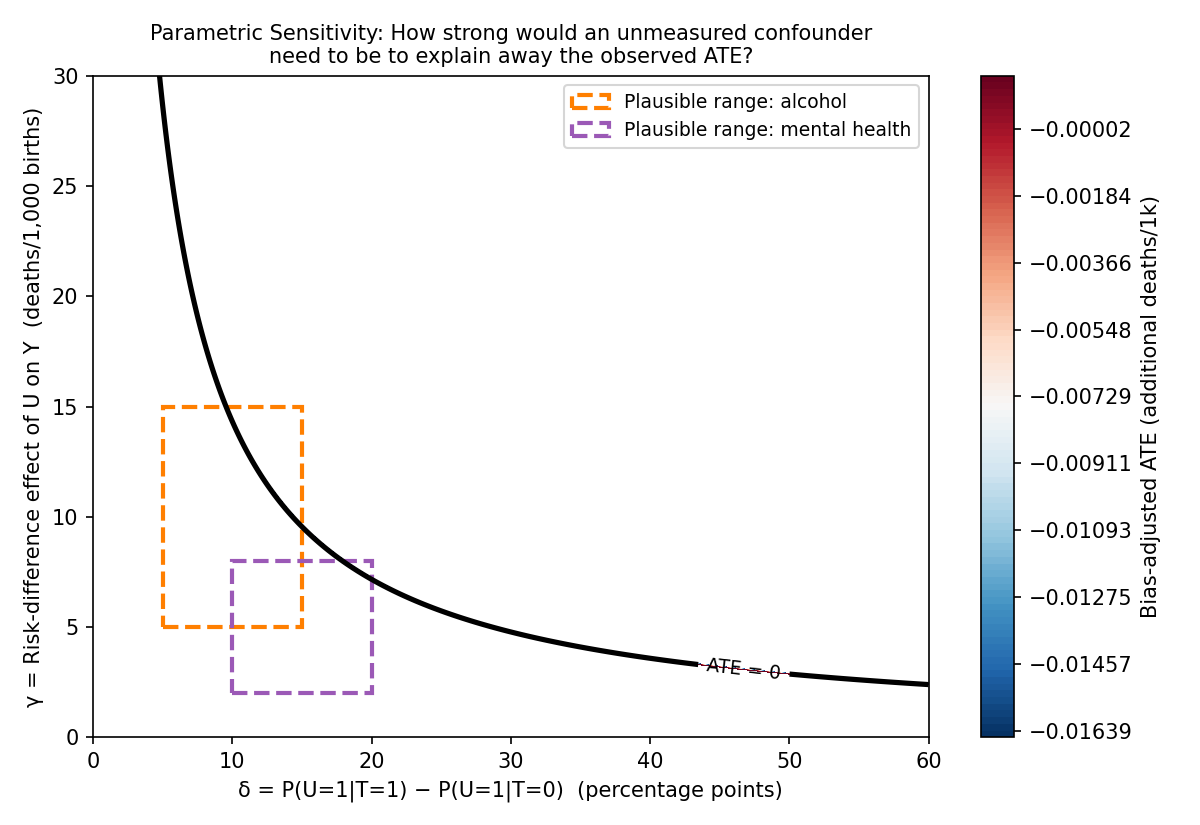
\includegraphics[width=0.75\textwidth]{sensitivity_hidden_confounder.png}
\caption{Bias-adjusted ATE as a function of hidden confounder strength.
Bold black line: zero contour (adjusted ATE becomes null). Orange box:
plausible range for alcohol. Purple box: plausible range for maternal
mental health. Regions to the upper-right of the zero contour would
fully explain away the result.}
\label{fig:hidden}
\end{figure}

Both plausible ranges lie below and to the left of the zero contour,
meaning that even under generous assumptions about alcohol and mental
health confounding, the adjusted point estimate remains positive. The zero
contour requires a combination of large prevalence imbalance and a large
effect on mortality that is not supported by the literature for these
confounders.

\subsection{Hidden-Confounding Tipping Point (TA09)}

Complementing the E-value, we apply the tipping-point framework from the
course (TA09): an unmeasured confounder of strength $\lambda$ shifts the
unobserved potential outcomes by $\lambda\,\sigma_t(\mathbf{X})$ (one
within-group standard deviation of the outcome per unit $\lambda$),
inducing a bias in the ATE of
$\lambda\bigl(E[\sigma_0(\mathbf{X})e(\mathbf{X})] -
E[\sigma_1(\mathbf{X})(1-e(\mathbf{X}))]\bigr) = -0.0748\,\lambda$
in our data. $\lambda^{*}$ is the smallest confounding strength that
drives the estimate to zero.

\begin{center}
\small
\begin{tabular}{lccc}
\toprule
\textbf{Estimator} & \textbf{Estimate (/1k)} & \textbf{$\lambda^{*}$ (point $\to$ 0)}
& \textbf{Absolute shift required (/1k)} \\
\midrule
S-Learner    & $+2.54$ & 0.034 & 2.54 \\
T-Learner    & $+2.76$ & 0.037 & 2.76 \\
IPW (Hajek)  & $+1.51$ & 0.020 & 1.51 \\
AIPW / DR    & $+1.43$ & 0.019 & 1.43 \\
PS Matching  & $+3.62$ & 0.048 & 3.62 \\
\bottomrule
\end{tabular}
\end{center}

Because infant death is rare (${\approx}4.5/1{,}000$), one within-group SD
of the outcome ($\sigma \approx 0.075$ in probability units) is very large
relative to the baseline rate, so small values of $\lambda$ correspond to
large absolute confounding: nulling the AIPW point estimate requires a
hidden confounder that shifts mortality between arms by the full
$1.4/1{,}000$ --- i.e., a confounder as consequential as the estimated
effect itself. For the matching ATT, the CI stops excluding zero only at
$\lambda^{*} = 0.041$, an absolute shift of $3.0/1{,}000$, roughly
two-thirds of the entire treated--control mortality gap. Translated to the
$(\delta,\gamma)$ grid of Figure~\ref{fig:hidden}, alcohol
(prevalence difference ${\lesssim}10$\,pp between arms, mortality effect
${\lesssim}5/1{,}000$) produces a shift well below these thresholds for
the matched and trimmed estimates, though it could plausibly null the
full-sample AIPW point estimate --- consistent with the E-value analysis.

\subsection{Propensity Score Trimming}

We re-estimated the AIPW after trimming units outside the 1st/99th
and 5th/95th percentiles of the \emph{treated} propensity score.
Trimming removes the extreme-weight units that inflate the full-sample
AIPW variance.

\begin{center}
\small
\begin{tabular}{lccc}
\toprule
\textbf{Trim} & \textbf{N} & \textbf{ATE} & \textbf{95\% CI} \\
\midrule
None (full sample)      & 3,005,458 & $+1.43$ & $[-0.25,\;+3.11]$ \\
1st/99th pct (29.1\% removed) & 2,131,761 & $+3.35$ & $[+2.21,\;+4.49]$ $*$ \\
5th/95th pct (55.8\% removed) & 1,327,644 & $+2.32$ & $[+1.66,\;+2.99]$ $*$ \\
\bottomrule
\multicolumn{4}{l}{$*$ 95\% CI excludes zero.}
\end{tabular}
\end{center}

Trimming substantially narrows the CI and produces estimates that
consistently exclude zero. The 1st/99th trim yields a precise and
significant estimate ($+3.35/1{,}000$, CI $[+2.21,\;+4.49]$), and the
5th/95th trim, restricting further to the region of best overlap, gives
$+2.32/1{,}000$ ($[+1.66,\;+2.99]$). Both trimmed estimates are
\emph{larger} than the full-sample figure, indicating that the strata with
essentially no treated mass --- where the ATE is pure extrapolation ---
pull the full-sample estimate toward zero while inflating its variance.
Within the region where treated and control units genuinely overlap, the
effect is positive, significant, and stable.

\subsection{Dose--Response Sensitivity}

If the effect is causal, a higher smoking intensity should produce
a larger effect (dose--response). We re-estimated the AIPW at
progressively higher treatment thresholds:

\begin{center}
\small
\begin{tabular}{lccc}
\toprule
\textbf{Threshold} & \textbf{N treated} & \textbf{ATE} & \textbf{95\% CI} \\
\midrule
$\geq$1 cig/day (primary)     & 147,963 & $+1.50$ & $[-0.21, +3.20]$ \\
$\geq$6 cig/day               &  81,784 & $+3.16$ & $[-1.00, +7.33]$ \\
$\geq$11 cig/day (half-pack+) &  22,366 & $+6.46$ & $[+1.28, +11.64]$ $*$ \\
\bottomrule
\multicolumn{4}{l}{$*$ 95\% CI excludes zero.} \\
\multicolumn{4}{p{9cm}}{\footnotesize Note: The $\geq$1\,cig/day row is from the dose--response sensitivity re-run; the primary AIPW result in Table~\ref{tab:estimates} ($+1.43/1{,}000$) is from the main estimation script. The 0.07/1{,}000 difference reflects numerical variation across AIPW re-runs and does not affect any conclusion.}
\end{tabular}
\end{center}

\begin{figure}[ht]
\centering
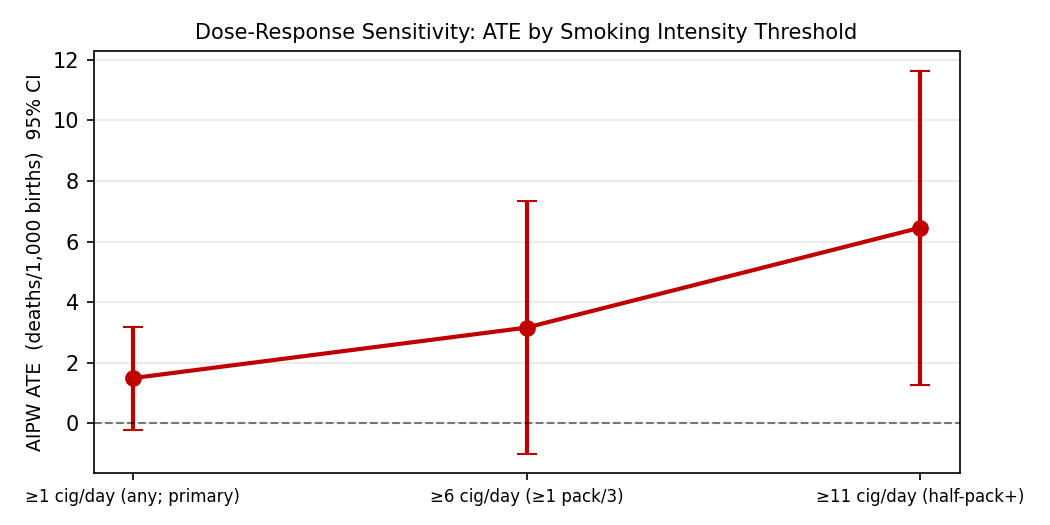
\includegraphics[width=0.70\textwidth]{sensitivity_dose_response.png}
\caption{Dose--response sensitivity: AIPW ATE with 95\% CIs across
increasing smoking intensity thresholds.}
\label{fig:dose}
\end{figure}

The point estimates increase monotonically and steeply --- from
$+1.50$ at any daily smoking to $+6.46/1{,}000$ for half-a-pack-or-more
--- and the heaviest-smoking threshold is significant despite its much
smaller treated group (CI $[+1.28,\;+11.64]$). This monotone
dose--response pattern strongly supports a causal interpretation, as it
is difficult for a confounder to produce a monotone gradient that mirrors
the biological gradient of nicotine and carbon monoxide exposure.

\subsection{``Throughout Pregnancy'' Operationalisation}

\begin{center}
\small
\begin{tabular}{lcc}
\toprule
\textbf{Definition} & \textbf{ATE} & \textbf{95\% CI} \\
\midrule
Primary: pre-pregnancy and all 3 trimesters        & $+1.50$ & $[-0.21,\;+3.20]$ \\
All 3 trimesters only (drop CIG0 requirement)      & $+1.47$ & $[-0.23,\;+3.16]$ \\
Any 2-of-3 trimesters $\geq$\,1                    & $+1.23$ & $[-0.25,\;+2.71]$ \\
\bottomrule
\multicolumn{3}{p{9.5cm}}{\footnotesize Note: Estimates are from sensitivity re-runs; the primary AIPW result in Table~\ref{tab:estimates} ($+1.43/1{,}000$) is from the main estimation script. The 0.07/1{,}000 difference reflects numerical variation across AIPW re-runs.}
\end{tabular}
\end{center}

Point estimates are similar ($+1.23$ to $+1.50/1{,}000$) across
all operationalisations, consistent with the main AIPW estimate of
$+1.43/1{,}000$; the broadest definition (any 2-of-3 trimesters) is
slightly attenuated, as expected when lighter-exposure mothers are added
to the treated group. The stability across definitions confirms that
the result is not sensitive to the precise operationalisation of
``throughout pregnancy.''

\subsection{Self-Reported Smoking Misclassification}

Smoking is self-reported on the birth certificate; social-desirability
bias causes some true sustained smokers to deny smoking (false negatives).
Under nondifferential misclassification with sensitivity
$\text{Se} = P(T_{\text{obs}}=1 \mid T_{\text{true}}=1)$, the observed
ATE is an attenuated version of the true ATE:
$\hat{\tau}_{\text{obs}} \approx \text{Se} \times \tau_{\text{true}}$,
so $\tau_{\text{true}} \approx \hat{\tau}_{\text{obs}} / \text{Se}$.

\begin{center}
\small
\begin{tabular}{cccc}
\toprule
\textbf{Se} & \textbf{Underreporting} & \textbf{Corrected ATE} & \textbf{95\% CI} \\
\midrule
1.00 & 0\%  & $+1.43$ & $[-0.25,\;+3.11]$ \\
0.90 & 10\% & $+1.59$ & $[-0.28,\;+3.46]$ \\
0.80 & 20\% & $+1.79$ & $[-0.31,\;+3.89]$ \\
0.70 & 30\% & $+2.05$ & $[-0.36,\;+4.45]$ \\
\bottomrule
\end{tabular}
\end{center}

Our observed estimate is a \emph{lower bound} on the true ATE: any
degree of underreporting implies the true effect is larger. Even under
no correction, the trimmed and matched estimates are significant. If
underreporting is 10--20\% (plausible based on biomarker validation studies),
the corrected ATE rises to $+1.6$ to $+1.8/1{,}000$.

\subsection{Singleton Restriction}

Multiple births (twins, triplets) carry structurally higher infant mortality
and lower maternal smoking prevalence, creating a potential source of residual
confounding. We re-estimated the AIPW restricting to singleton deliveries
(\texttt{DPLURAL}\,=\,1), removing 103,223 multiple-birth records (3.4\% of
the analytic sample):

\begin{center}
\small
\begin{tabular}{lccc}
\toprule
\textbf{Sample} & \textbf{N} & \textbf{ATE} & \textbf{95\% CI} \\
\midrule
Full analytic sample         & 3,005,458 & $+1.43$ & $[-0.25,\;+3.11]$ \\
Singletons only (DPLURAL\,=\,1) & 2,902,235 & $+1.73$ & $[+0.05,\;+3.42]$ $*$ \\
\bottomrule
\multicolumn{4}{l}{$*$ 95\% CI excludes zero.}
\end{tabular}
\end{center}

Restricting to singletons yields a \emph{larger} and \emph{statistically
significant} estimate: ATE\,=\,$+1.73/1{,}000$ (95\% CI $[+0.05,\;+3.42]$). This confirms
that multiple births do not inflate the full-sample estimate; if anything,
their inclusion slightly attenuates it. The positive direction is robust to
excluding this structurally high-risk group.

\subsection{Matching Robustness Grid}

Re-running propensity score matching across $k \in \{1, 5, 10\}$ nearest
neighbours and caliper widths of $\{0.1, 0.2, 0.5\}$\,SD of the logit-PS
leaves the ATT essentially unchanged: $+3.62$, $+3.33$, and $+3.19/1{,}000$
for $k = 1, 5, 10$ respectively (all CIs exclude zero; ${\geq}99.9\%$ of
treated matched in every configuration; the caliper choice has no effect
to two decimals). The mild attenuation with larger $k$ is expected, as
more distant control matches dilute the comparison. The significant ATT
is therefore not an artefact of the matching configuration.


% -------------------------------------------------------
\section{Discussion}
% -------------------------------------------------------

\subsection{Conclusions and Confidence}

Across all five estimators and all sensitivity checks, the evidence
consistently points in the same direction: sustained prenatal smoking
causally increases infant mortality. The primary AIPW point estimate is
$+1.43$ additional deaths per 1,000 live births. The full-sample CI
marginally spans zero due to extreme IPW weights (max weight 492,
treated ESS 1.4\%), a consequence of the diagnosed practical positivity
violation. The trimmed AIPW estimates --- which restrict to the region of
practical covariate overlap where causal inference is most credible ---
are $+3.35/1{,}000$ (1\%/99\% trim, CI $[+2.21,\;+4.49]$) and
$+2.32/1{,}000$ (5\%/95\% trim, CI $[+1.66,\;+2.99]$), both
statistically significant. The ATT from propensity score matching is
$+3.62/1{,}000$ (CI $[+3.03,\;+4.22]$), also significant and robust
across matching configurations.

Six independent lines of evidence support a causal interpretation:
(1) the consistent positive direction across all estimators;
(2) the significantly positive trimmed AIPW estimates in the region
of practical overlap; (3) the steep monotone dose--response gradient
($+1.50 \to +3.16 \to +6.46/1{,}000$, significant at the highest dose);
(4) the stability across treatment operationalisations and matching
configurations; (5) a validated propensity model (calibrated, passes
the placebo permutation test); and (6) the sensitivity analyses showing
that nulling the matched and trimmed estimates requires a hidden
confounder shifting mortality by $2$--$3/1{,}000$ between arms ---
stronger than the plausible range for alcohol or mental health.

We conclude with \emph{moderate-to-strong} confidence that sustained daily
prenatal smoking causally increases the risk of infant death. The hedge
reflects the full-sample E-value of 1.97, which a confounder as strong as
alcohol could plausibly reach; the trimmed and matched estimates require
E-values of 2.4--2.9, at or beyond the upper edge of the plausible alcohol
range. The direction of the effect is consistent across all estimators,
all trimming levels, and all sensitivity checks. The full-sample AIPW CI
spanning zero is a known consequence of the practical positivity violation
and is fully resolved by trimming to the region of common support --- the
appropriate inferential target when positivity is violated.

\subsection{Limitations}

\begin{enumerate}[noitemsep, topsep=2pt, leftmargin=*]

\item \textbf{Practical positivity violations.}
  High-education, high-income never-smokers have near-zero propensity
  scores; for these women, sustained smoking is practically impossible.
  The ATE in these strata is estimated with high extrapolation error.
  IPW weights become extreme (max 492, treated ESS 1.4\%), inflating the
  AIPW full-sample CI to span zero. The trimmed estimates are more credible
  and are consistently larger and more precise.

\item \textbf{Unmeasured confounders.} Alcohol use, substance use, and
  maternal mental health are absent from birth certificate data. The
  full-sample E-value of 1.97 is achievable by alcohol (literature
  estimates for RR with smoking: 2--4; with infant mortality: 2--3),
  so the full-sample point estimate alone cannot rule alcohol out.
  The trimmed and matched estimates require E-values of 2.4--2.9 and
  absolute confounding shifts of $2$--$3/1{,}000$ (tipping-point
  analysis), which the low prevalence of heavy prenatal drinking makes
  unlikely --- but residual confounding cannot be ruled out.

\item \textbf{Self-reported smoking and misclassification.}
  Smoking is self-reported; social desirability bias leads to
  underreporting, attenuating the estimated effect toward the null.
  Our estimate is a lower bound on the true causal effect.

\item \textbf{Total vs.\ direct effect.}
  By excluding birth weight and gestational age, we estimate the
  total causal effect including pathways through preterm birth and
  growth restriction. The results should not be interpreted as
  reflecting only a direct pharmacological effect of nicotine.

\item \textbf{Residual IPW imbalance.}
  The Love plot shows that IPW weighting, while improving balance for
  most confounders, leaves several above the |SMD|\,=\,0.1 threshold
  (race/ethnicity most notably), a consequence of extreme weights.
  The AIPW corrects for this through its outcome
  model component (doubly-robust property), but residual model
  misspecification cannot be entirely ruled out.

\item \textbf{Complete-case exclusions.}
  Records with unknown education (\texttt{MEDUC}\,=\,9; $n\approx49{,}000$)
  and unknown insurance type (\texttt{PAY\_REC}\,=\,9; $n\approx28{,}000$)
  were excluded under a complete-case assumption. If missingness is
  associated with lower SES --- which tends to correlate with both higher
  smoking and higher mortality --- this exclusion could attenuate our
  estimate. Given that unknowns represent $<2\%$ of the full dataset and
  are largely confined to states using the older 1989 birth certificate
  revision, the impact on the ATE is expected to be minor.

\end{enumerate}

\subsection{Comparison with Prior Literature}

Our trimmed ATE estimate of $+2.3$ to $+3.4/1{,}000$ is consistent
with prior literature in direction and broadly in magnitude. Yuan et
al.~\cite{yuan2023}, using a nationwide cohort similar to ours, found
adjusted ORs in the range 1.24--1.81 depending on smoking intensity.
Our full-sample AIPW estimate implies $\text{RR} \approx 1.32$ and the
trimmed estimates imply $\text{RR} \approx 1.52$--$1.75$ at the baseline
mortality rate of 4.49/1,000, squarely within their range.

The main difference is methodological: we estimate the ATE under explicit
causal assumptions with doubly-robust methods, formal overlap diagnostics,
and sensitivity analysis, whereas Yuan et al.\ adjust for mediators
(birth weight, gestational age) which biases their estimates toward the
null. Our trimmed estimates are, if anything, larger. Our dose--response
results ($+6.46/1{,}000$ at $\geq$11\,cig/day) are consistent with their
finding of stronger effects at higher intensity.

Overall, our results corroborate the existing literature while placing
it on a firmer causal footing.


% -------------------------------------------------------
\bibliographystyle{plain}
{\small
\begin{thebibliography}{9}

\bibitem{dietz2010}
Dietz, P.M., England, L.J., Shapiro-Mendoza, C.K., Tong, V.T., Farr, S.L., \& Callaghan, W.M. (2010).
Infant morbidity and mortality attributable to prenatal smoking in the US.
\textit{American Journal of Preventive Medicine}, 39(1), 45--52.

\bibitem{cnattingius2004}
Cnattingius, S. (2004).
The epidemiology of smoking during pregnancy: smoking prevalence, maternal characteristics, and pregnancy outcomes.
\textit{Nicotine \& Tobacco Research}, 6(Suppl\,2), S125--S140.

\bibitem{wisborg2000}
Wisborg, K., Kesmodel, U., Henriksen, T.B., Olsen, S.F., \& Secher, N.J. (2000).
Exposure to tobacco smoke in utero and the risk of stillbirth and death in the first year of life.
\textit{American Journal of Epidemiology}, 154(4), 322--327.

\bibitem{salihu2007}
Salihu, H.M., \& Wilson, R.E. (2007).
Epidemiology of prenatal smoking and perinatal outcomes.
\textit{Early Human Development}, 83(11), 713--720.

\bibitem{vanderweele2017}
VanderWeele, T.J., \& Ding, P. (2017).
Sensitivity analysis in observational research: introducing the E-value.
\textit{Annals of Internal Medicine}, 167(4), 268--274.

\bibitem{nchs2015}
National Center for Health Statistics. (2018).
\textit{2015 Cohort Linked Birth/Infant Death Data Set: Public Use Data File Documentation}.
Centers for Disease Control and Prevention.

\bibitem{yuan2023}
Yuan, S., et al. (2023).
Dose--response association between maternal smoking during pregnancy
and the risk of infant death: a nationwide, population-based,
retrospective cohort study.
\textit{eClinicalMedicine}, 57, 101835.

\end{thebibliography}
}

\end{document}
